
\let\negmedspace\undefined
\let\negthickspace\undefined
\documentclass[journal]{IEEEtran}
\usepackage[a5paper, margin=10mm, onecolumn]{geometry}
%\usepackage{lmodern} % Ensure lmodern is loaded for pdflatex
\usepackage{tfrupee} % Include tfrupee package

\setlength{\headheight}{1cm} % Set the height of the header box
\setlength{\headsep}{0mm}     % Set the distance between the header box and the top of the text

\usepackage{gvv-book}
\usepackage{gvv}
\usepackage{cite}
\usepackage{amsmath,amssymb,amsfonts,amsthm}
\usepackage{algorithmic}
\usepackage{graphicx}
\usepackage{textcomp}
\usepackage{xcolor}
\usepackage{txfonts}
\usepackage{listings}
\usepackage{enumitem}
\usepackage{mathtools}
\usepackage{gensymb}
\usepackage{comment}
\usepackage[breaklinks=true]{hyperref}
\usepackage{tkz-euclide} 
\usepackage{listings}
% \usepackage{gvv}                                        
\def\inputGnumericTable{}                                 
\usepackage[latin1]{inputenc}                                
\usepackage{color}                                            
\usepackage{array}                                            
\usepackage{longtable}                                       
\usepackage{calc}                                             
\usepackage{multirow}                                         
\usepackage{hhline}                                           
\usepackage{ifthen}                                           
\usepackage{lscape}
\begin{document}

\bibliographystyle{IEEEtran}
\vspace{3cm}

\title{
9 - Intersection of Conics \\
\large EE1030:Matrix Theory
}
\author{Gajjarapu Satyanarayana\\AI24BTECH11009
}
% \maketitle
% \newpage
% \bigskip
{\let\newpage\relax\maketitle}

\renewcommand{\thefigure}{\theenumi}
\renewcommand{\thetable}{\theenumi}



\numberwithin{equation}{enumi}
\numberwithin{figure}{enumi}
\renewcommand{\thetable}{\theenumi}


\textbf{Question}:9.3.21\\
If the area of the region bounded by the line $y = mx$ and the curve $x^2 = y$ is $\frac{32}{3}$ sq. units, then find the positive value of $m$, using integration. \hfill(12, 2022)
\\
\textbf{Solution:}
\renewcommand{\tablename}{Table 9.3.21.1}
\begin{table}[h!]
  \centering
  \begin{tabular}[12pt]{ |c| c|}
    \hline
    \textbf{Variables} & \textbf{Description}\\ 
    \hline
    $\textbf{V}_1, \vec{u}_1, f_1$ & Parameters of the parabola $y^2 = 4x$ \\
    \hline
     $\textbf{V}_2, \vec{u}_2, f_2$ & Parameters of the circle $4x^2 + 4xy^2 = 9$ \\
    \hline
    $\vec{x}^\intercal\brak{\textbf{V}_1 + \mu\textbf{V}_2}\vec{x} + 2\brak{\vec{u}_1 + \mu\vec{u}_2}^\intercal\vec{x} + \brak{f_1 + \mu f_2}$ & Intersection of two conics \\
    \hline
    \end{tabular}


  \caption{Variables and their description}
\end{table}
\\
The parameters of the given line equation are
\begin{align}
\vec{h} = \myvec{0 \\ 0}, \vec{m} = \myvec{1 \\ m}
\end{align}
The parameters of given curve when expressed as a conic
\begin{align}
  \textbf{V} = \myvec{1 & 0 \\0 & 0},\vec{u} = \myvec{0 \\ -\frac{1}{2}},f = 0 
\end{align}
Using these parameters,
\begin{align}
    g(\vec{h}) & = 0 \\
    \kappa_i & = \frac{1}{1}\brak{-\myvec{1 & m}\myvec{0 \\ -\frac{1}{2}} \pm \myvec{1 & m}\myvec{0 \\ -\frac{1}{2}}} \\
    \kappa_1 & = 0, \kappa_2 = m
    \end{align}
The points of intersection of  line with conic are given by
\begin{align}
    \vec{x}_i & = \vec{h} + \kappa_i\vec{m} \\
    \vec{x}_1 & = \myvec{0 \\ 0} + 0\myvec{1 \\ m} \\
    \vec{x}_1 & = \myvec{0 \\ 0} \\
    \vec{x}_2 & = \myvec{0 \\ 0} + m\myvec{1 \\ m} \\
    \vec{x}_2 & = \myvec{m \\ m^2}
\end{align}
The area bounded by the curve and the line is $\frac{32}{3}$
\begin{align}
   \int_{0}^{m} (mx - x^2)dx & = \frac{32}{3} \\
   \sbrak{\frac{mx^2}{2} - \frac{x^3}{3}}_{0}^{m} & = \frac{32}{3} \\
   \frac{m^3}{2} - \frac{m^3}{3} & = \frac{32}{3} \\
   m^3 & = 64 \\
   m & = 4
   \end{align}
   \begin{figure}[h!]
   \centering
   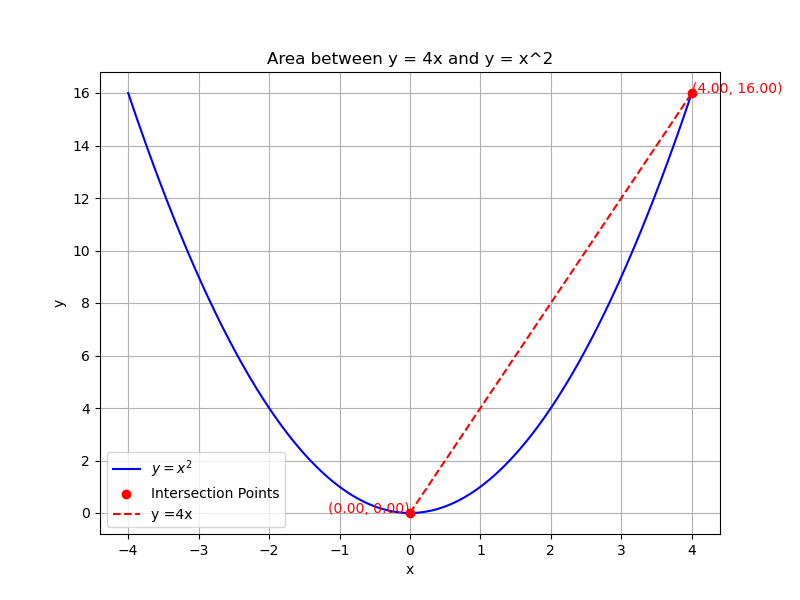
\includegraphics[width=0.7\linewidth]{figs/parab.png}
	\caption{Line and Parabola}
   \end{figure}
\end{document}

